%%%%%%%%%%%%%%%%%%%%%%%%%%%%%%%%%%%%%
%                                   %
% Compile with XeLaTeX and biber    %
%                                   %
% Questions or comments:            %
%                                   %
% joshua dot mcneill at uga dot edu %
%                                   %
%%%%%%%%%%%%%%%%%%%%%%%%%%%%%%%%%%%%%

\documentclass{beamer}
  % Read in standard preamble (cosmetic stuff)
  %%%%%%%%%%%%%%%%%%%%%%%%%%%%%%%%%%%%%%%%%%%%%%%%%%%%%%%%%%%%%%%%
% This is a standard preamble used in for all slide documents. %
% It basically contains cosmetic settings.                     %
%                                                              %
% Joshua McNeill                                               %
% joshua dot mcneill at uga dot edu                            %
%%%%%%%%%%%%%%%%%%%%%%%%%%%%%%%%%%%%%%%%%%%%%%%%%%%%%%%%%%%%%%%%

% Beamer settings
% \usetheme{Berkeley}
\usetheme{CambridgeUS}
% \usecolortheme{dove}
% \usecolortheme{rose}
\usecolortheme{seagull}
\usefonttheme{professionalfonts}
\usefonttheme{serif}
\setbeamertemplate{bibliography item}{}

% Packages and settings
\usepackage{fontspec}
  \setmainfont{Charis SIL}
\usepackage{hyperref}
  \hypersetup{colorlinks=true,
              allcolors=blue}
\usepackage{graphicx}
  \graphicspath{{../../figures/}}
\usepackage[normalem]{ulem}
\usepackage{enumerate}

% Document information
\author{M. McNeill}
\title[FREN2001]{Français 2001}
\institute{\url{joshua.mcneill@uga.edu}}
\date{}

%% Custom commands
% Lexical items
\newcommand{\lexi}[1]{\textit{#1}}
% Gloss
\newcommand{\gloss}[1]{`#1'}
\newcommand{\tinygloss}[1]{{\tiny`#1'}}
% Orthographic representations
\newcommand{\orth}[1]{$\langle$#1$\rangle$}
% Utterances (pragmatics)
\newcommand{\uttr}[1]{`#1'}
% Sentences (pragmatics)
\newcommand{\sent}[1]{\textit{#1}}
% Base dir for definitions
\newcommand{\defs}{../definitions}


  % Packages and settings

  % Document information
  \subtitle[Chemin et \lexi{que}]{Indiquer le chemin et le pronom relatif \lexi{que}}

\begin{document}
  % Read in the standard intro slides (title page and table of contents)
  \begin{frame}
    \titlepage
    \tiny{Office: % Basically a variable for office hours location
Gilbert 121\\
          Office hours: % Basically a variable for office hours
 lundi, mercredi, vendredi 10:10--11:10
}
  \end{frame}

  \begin{frame}{Où est-ce que tu arriveras?}
    \small
    \begin{columns}
      \column{0.3\textwidth}

        \only<1>{
          Tu commenceras à la gare.
        }

        \only<2>{
          Tu traverseras le boulevard Heurteloup.
        }

        \only<3>{
          Tu prendras la rue Bernard Palissy et tu continueras tout droit.
        }

        \only<4>{
          À la place François Sicard, tu tourneras à droite.
        }

        \only<5-6>{
          Où seras-tu? \underline{\uncover<6>{le musée des beaux-arts}} et \underline{\uncover<6>{la cathédrale}}
        }

        \only<7>{
          Tu commenceras à la gare.
        }

        \only<8>{
          Tu tourneras à gauche dans le boulevard Heurteloup jusqu'à la place Jean Jaurès.
        }

        \only<9>{
          Ensuite, tu tourneras à droite dans la rue Nationale et continueras tout droit jusqu'à la rue des Tanneurs tout près de la Loire.
        }

        \only<10>{
          Tu tourneras à gauche et voilà ce sera sur ta droite.
        }

        \only<11-12>{
          Où seras-tu? \underline{\uncover<12>{la faculté}}
        }

        \only<13>{
          Tu commenceras à la gare.
        }

        \only<14>{
          Le plus facile, c'est de suivre la rue Nationale jusqu'à la Loire et de prendre la rue des Tanneurs juste avant le quai du Pont Neuf.
        }

        \only<15>{
          Ensuite, tu tourneras à gauche en face de la fac dans une petite rue piétonnière \gloss{pedestrian street}.
        }

        \only<16-17>{
          Où seras-tu? \underline{\uncover<17>{la place Plumereau}}
        }

        \only<18>{
          Tu commenceras à la gare.
        }

        \only<19>{
          Traverse le boulevard Heurteloup, prends la rue de Buffon, tourne à gauche dans la rue de la Scellerie et continue tout droit.
        }

        \only<20>{
          Traverse la rue Nationale.
        }

        \only<21>{
          Suis la rue des Halles.
        }

        \only<22>{
          C'est au bout \gloss{at the end} sur ta gauche.
        }

        \only<23-24>{
          Où seras-tu? \underline{\uncover<24>{les halles}}
        }
      \column{0.7\textwidth}
        \begin{minipage}[c][0.8\textheight]{\linewidth}
          \begin{center}
            \only<1-5,7-11,13-16,18-23>{
              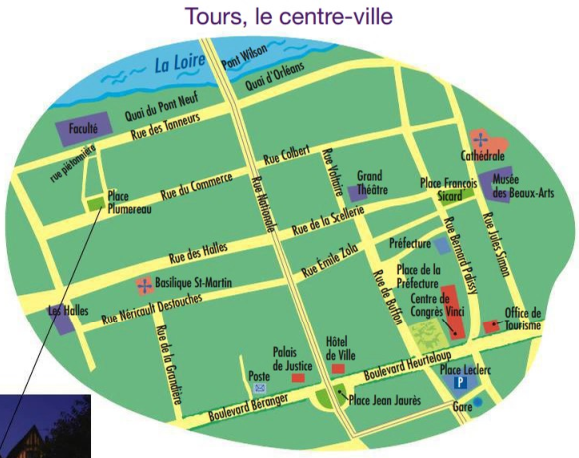
\includegraphics[scale=0.53]{plan_de_tours.png}
            }
            \only<6>{
              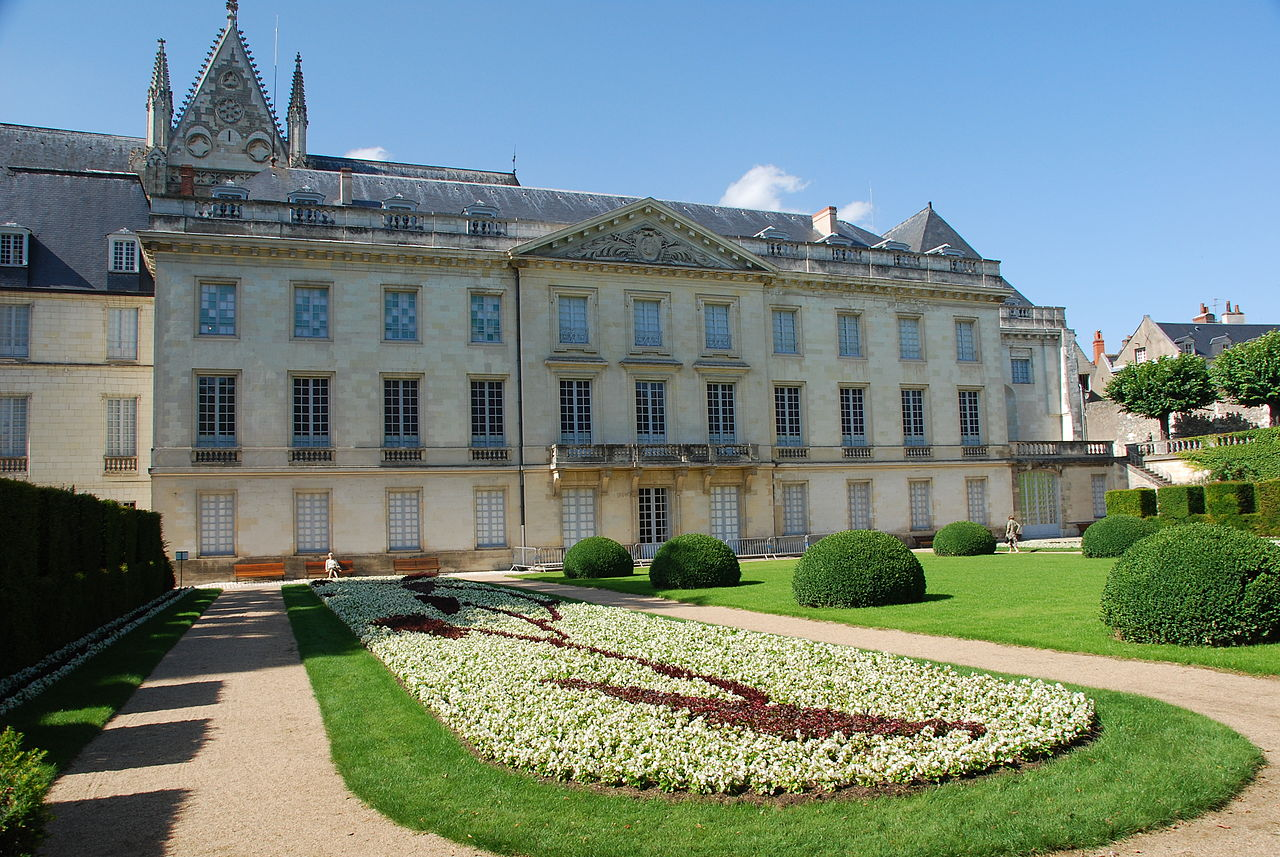
\includegraphics[scale=0.45]{beaux-arts.jpg}
              \includegraphics[scale=0.06]{cathédrale.jpg}
            }
            \only<12>{
              
\includegraphics[scale=0.3]{faculté.jpg}
            }
            \only<17>{
              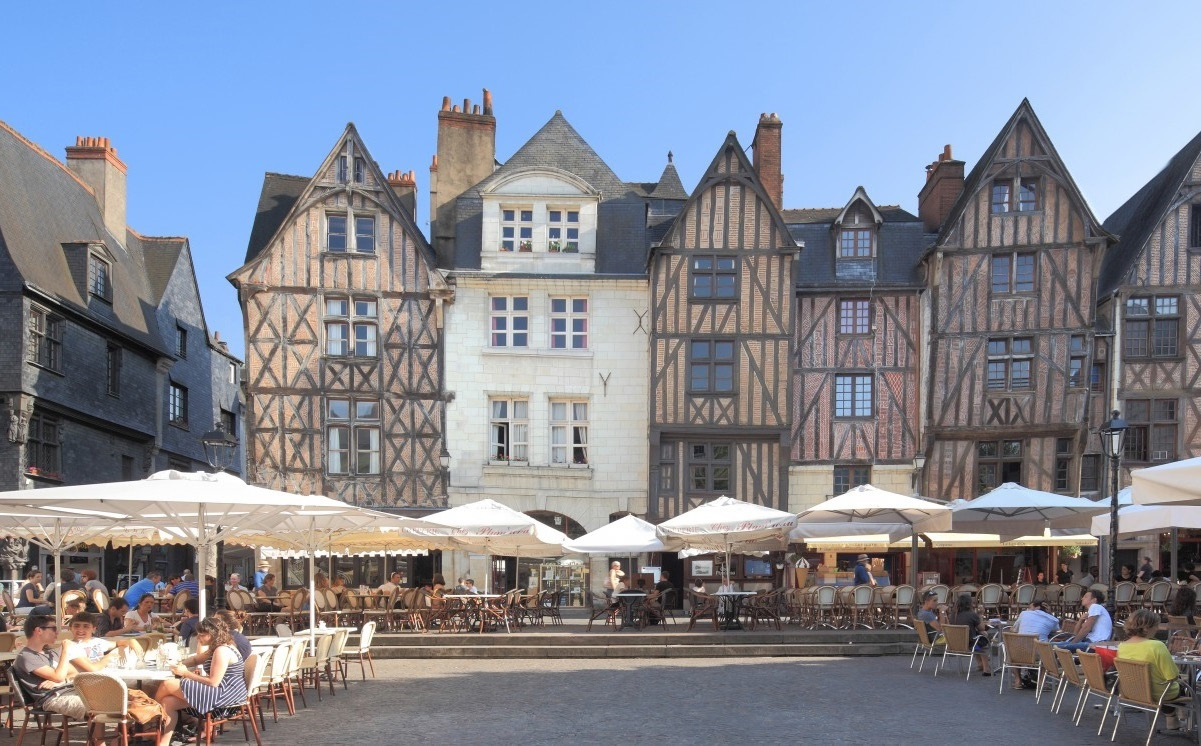
\includegraphics[scale=0.2]{plumereau.jpg}
            }
            \only<24>{
              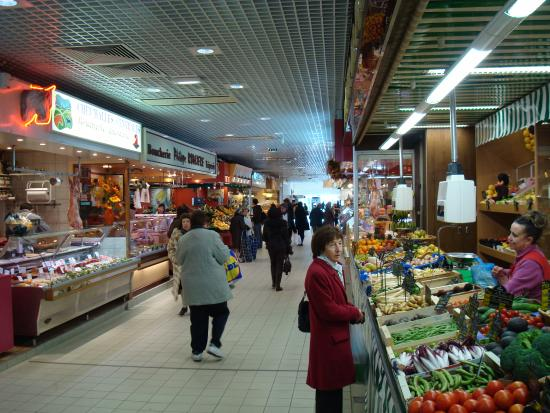
\includegraphics[scale=0.38]{halles.jpg}
            }
          \end{center}
        \end{minipage}
    \end{columns}
  \end{frame}

  \begin{frame}{}
    \begin{center}
      \Large Quiz
    \end{center}
  \end{frame}

  \begin{frame}{Le mot juste}
    Avec un/e partenaire, utilisez des pronoms relatifs pour définir les mots suivants.
    Écrivez vos définitions sur un papier.
    \begin{description}
      \item[] \textbf{Modèle:} \textit{une auberge de jeunesse}
      \item[E1:] C'est un endroit \alert{où} les jeunes peuvent rencontrer d'autres jeunes voyageurs.
      \item[E2:] C'est aussi un logement \alert{qui} ne coûte pas très cher.
    \end{description}
    \begin{columns}[t]
      \column{0.5\textwidth}
        \begin{enumerate}
          \item un gîte rural
          \item un spectacle son et lumière
          \item une visite guidée
          \item un musée
        \end{enumerate}
      \column{0.5\textwidth}
        \begin{enumerate}
          \setcounter{enumi}{4}
          \item un office de tourisme
          \item une agence de voyages
          \item un/e réceptionniste
          \item un/e agent de police
        \end{enumerate}
    \end{columns}
  \end{frame}

  \begin{frame}{}
    \begin{center}
      \Large Questions?
    \end{center}
  \end{frame}
\end{document}
